\documentclass[
  12pt,
  handout,
  aspectratio=1610,
  mathserif
]{beamer}

\usepackage{gmsh}
\usepackage{booktabs}

\graphicspath{{./data_general_overview/}{../figures/}}
\addmediapath{{./data_general_overview/}}

\usetikzlibrary{arrows.meta,positioning}

\definecolor{gmshgreen}{RGB}{0,145,105}
\definecolor{softgray}{RGB}{245,246,248}

\lstset{
  basicstyle=\ttfamily\scriptsize,
  columns=fullflexible,
  keepspaces=true,
  showstringspaces=false,
  breaklines=true
}

\title{
\includegraphics[width=2.5cm]{gmsh.png}\\
  Boundary Layers in Gmsh}
\author{C. Geuzaine and J.-F. Remacle}
\institute{Universit\'e de Li\`ege and Universit\'e catholique de Louvain}
\date{\today}

\begin{document}

\begin{frame}[plain]
  \titlepage
\end{frame}

\begin{frame}{Philosophy}
  \begin{columns}[T,totalwidth=\textwidth]
    \begin{column}{0.56\textwidth}
      \begin{itemize}
        \item \texttt{BoundaryLayer} is a plugin: it is applied after the usual Gmsh meshing flow.
        \item We start from a healthy, watertight mesh and keep its topology.
        \item The plugin creates zero-thickness layer elements on selected curves or surfaces.
        \item A robust Winslow untangler pushes the layer into the existing mesh.
        \item The pushed macro layer is then split into the requested graded layers.
        \item Near-wall layers keep the prescribed size; farther away, the mesh adapts to available space.
      \end{itemize}
    \end{column}
    \begin{column}{0.40\textwidth}
      \centering
      \begin{tikzpicture}[
        node distance=0.55cm,
        flowbox/.style={draw=myblue,rounded corners=2pt,thick,align=center,
                        minimum width=3.8cm,minimum height=0.72cm,fill=softgray},
        arrow/.style={-{Latex[length=2mm]},thick,gmshgreen}
      ]
        \node[flowbox] (m0) {valid Gmsh mesh};
        \node[flowbox,below=of m0] (m1) {zero-thickness\\layer topology};
        \node[flowbox,below=of m1] (m2) {Winslow push\\and untangle};
        \node[flowbox,below=of m2] (m3) {split into\\graded layers};
        \node[flowbox,below=of m3] (m4) {optional high order};
        \draw[arrow] (m0) -- (m1);
        \draw[arrow] (m1) -- (m2);
        \draw[arrow] (m2) -- (m3);
        \draw[arrow] (m3) -- (m4);
      \end{tikzpicture}
    \end{column}
  \end{columns}
\end{frame}

\begin{frame}[fragile]{Current Controls}
  \begin{columns}[T,totalwidth=\textwidth]
    \begin{column}{0.42\textwidth}
      Main plugin inputs:
      \begin{itemize}
        \item \texttt{Surfaces}, \texttt{Curves} in 2D.
        \item \texttt{Volumes}, \texttt{Surfaces} in 3D.
        \item \texttt{Thickness}: total requested layer thickness.
        \item \texttt{Size}: first layer size.
        \item \texttt{Ratio}: geometric growth factor.
        \item \texttt{SmoothingLayers}: affected background rings.
        \item \texttt{HighOrder}: optional curved layer construction.
      \end{itemize}
    \end{column}
    \begin{column}{0.55\textwidth}
      \begin{lstlisting}[language=Python]
import gmsh

gmsh.initialize()
gmsh.open("3cw.geo")
gmsh.model.mesh.generate(2)

gmsh.plugin.setString("BoundaryLayer", "Surfaces", "16")
gmsh.plugin.setString("BoundaryLayer", "Curves", "1,2,3,4,5,6,7")

gmsh.plugin.setNumber("BoundaryLayer", "Thickness", 40.0)
gmsh.plugin.setNumber("BoundaryLayer", "Size", 0.3)
gmsh.plugin.setNumber("BoundaryLayer", "Ratio", 1.5)
gmsh.plugin.setNumber("BoundaryLayer", "SmoothingLayers", 5)
gmsh.plugin.setNumber("BoundaryLayer", "HighOrder", 2)

gmsh.plugin.run("BoundaryLayer")
gmsh.write("3cw_bl.msh")
      \end{lstlisting}
    \end{column}
  \end{columns}
\end{frame}

\begin{frame}{High Order as Post-Processing}
  \begin{columns}[T,totalwidth=\textwidth]
    \begin{column}{0.49\textwidth}
      \centering
      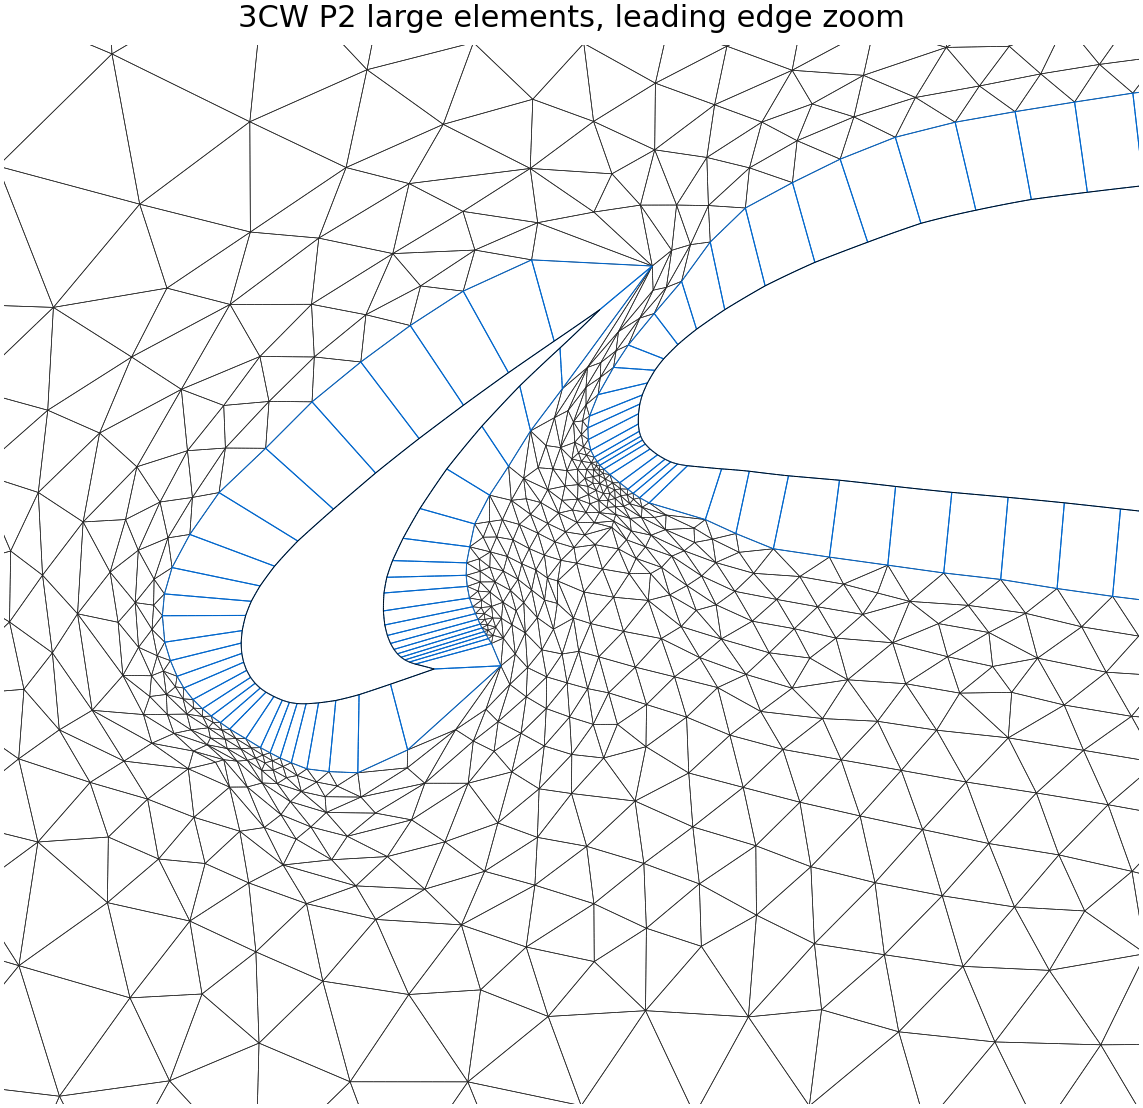
\includegraphics[height=0.55\textheight]{3cw_bl_p2_unsplit_leading_edge.png}

      \vspace{0.2cm}
      {\small The high-order pass first curves and untangles a large macro
      layer. The geometry is captured before the final split.}
    \end{column}
    \begin{column}{0.49\textwidth}
      \centering
      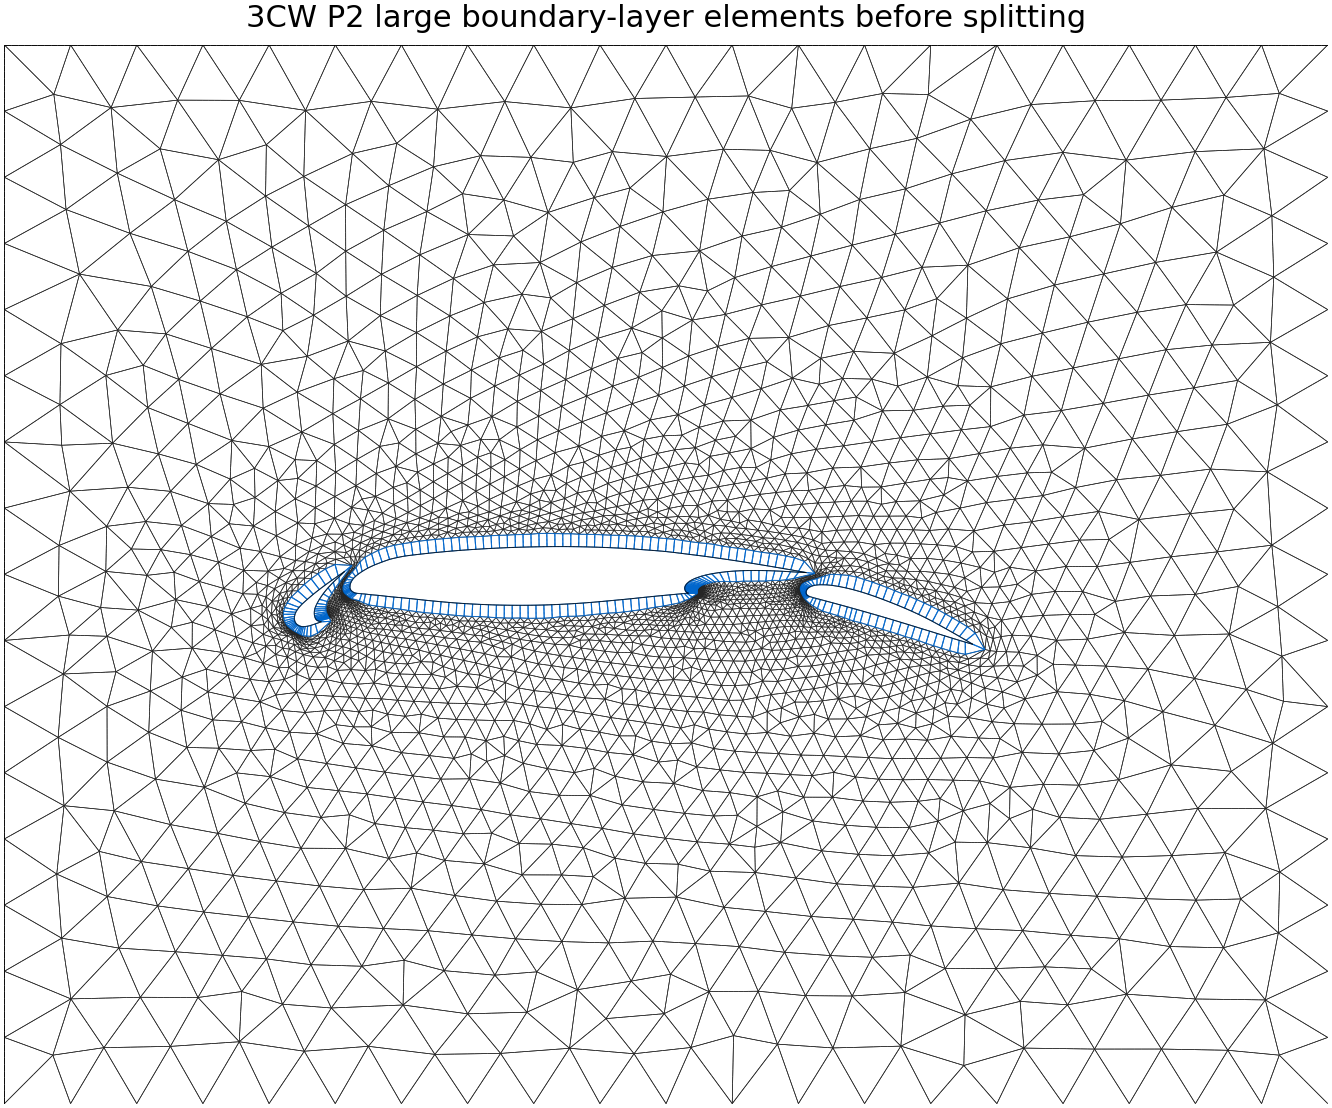
\includegraphics[height=0.55\textheight]{3cw_bl_p2_unsplit.png}

      \vspace{0.2cm}
      {\small The split is then performed in reference space: curvature is
      inherited cheaply and the boundary-layer topology stays consistent.}
    \end{column}
  \end{columns}
\end{frame}

\begin{frame}{3CW: Thickness Control}
  \begin{columns}[T,totalwidth=\textwidth]
    \begin{column}{0.53\textwidth}
      \centering
      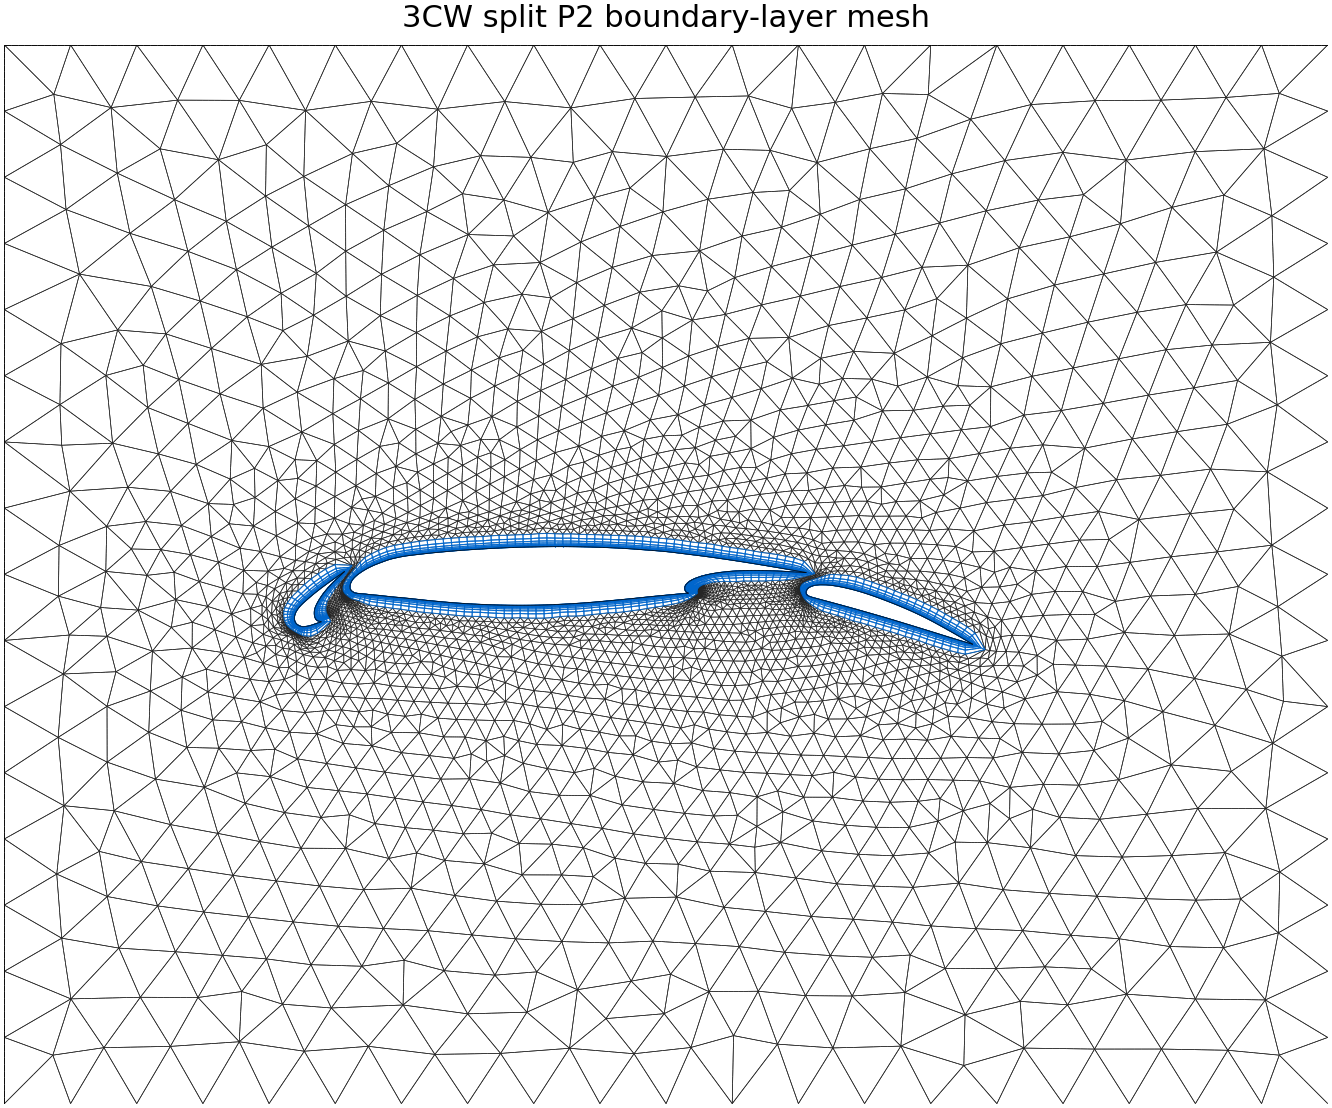
\includegraphics[height=0.55\textheight]{3cw_bl.png}
    \end{column}
    \begin{column}{0.43\textwidth}
      \centering
      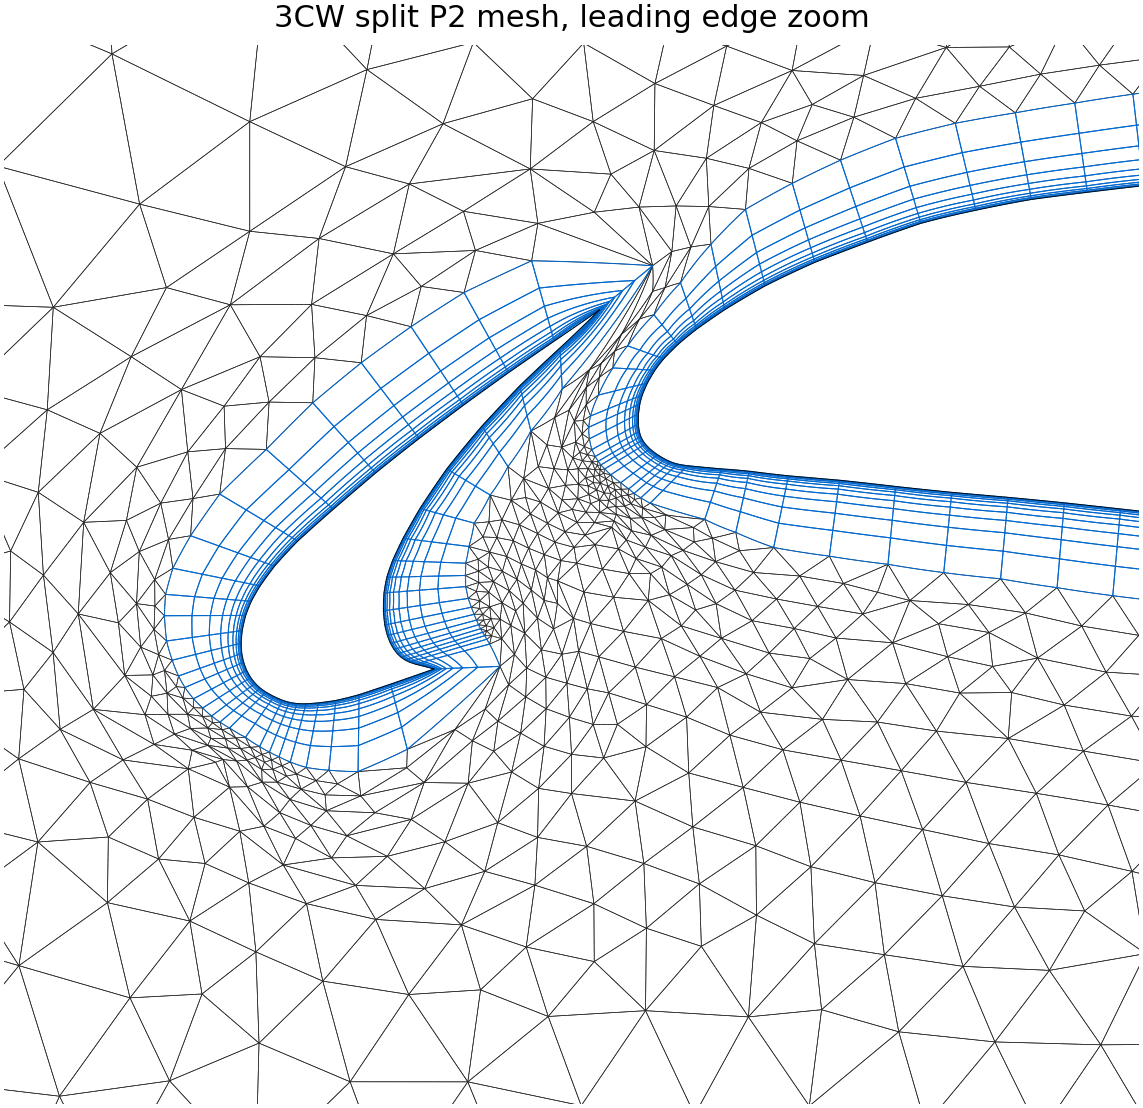
\includegraphics[height=0.55\textheight]{3cw_bl_leading_edge.png}
    \end{column}
  \end{columns}
  \vspace{0.12cm}
  \small
  The plugin first pushes a zero-thickness layer into the existing mesh, then
  splits it into the requested cells. The first layers keep the prescribed size;
  farther away the surrounding triangles adapt to the available space.
\end{frame}

\begin{frame}{RAE2822: RANS Sanity Check}
  \begin{columns}[T,totalwidth=\textwidth]
    \begin{column}{0.62\textwidth}
      \centering
      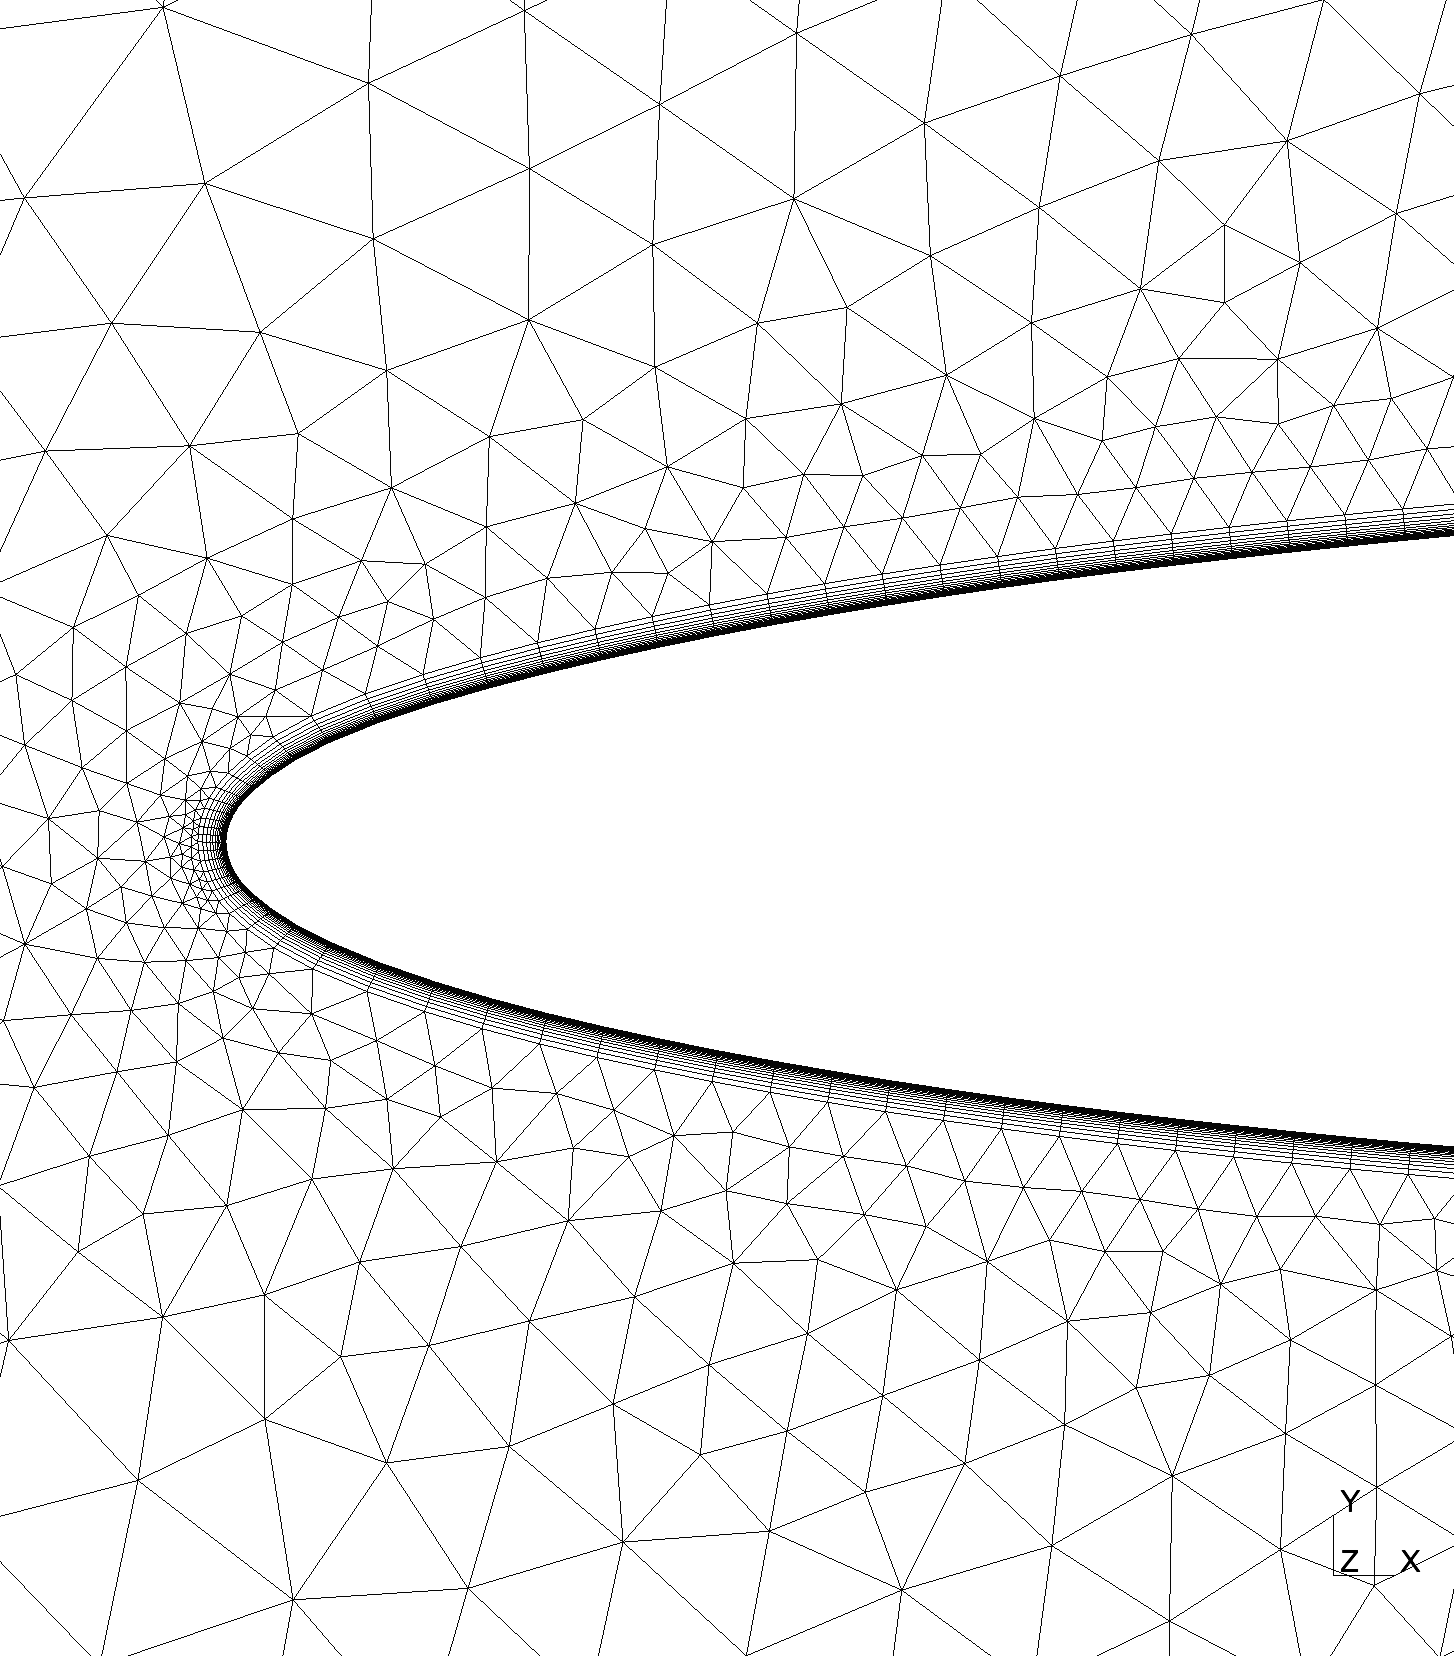
\includegraphics[height=0.70\textheight]{rae2822_mesh1.png}\\[-0.05cm]
      {\scriptsize RAE2822 boundary-layer mesh used for the SU2 run}
    \end{column}
    \begin{column}{0.34\textwidth}
      {\small \(M_\infty=0.734,\ \alpha=2.8^\circ,\ Re=6.5\times 10^6\)}
      \vspace{0.2cm}

      \scriptsize
      \begin{tabular}{lcc}
        \toprule
        Case & \(C_L\) & \(C_D\) \\
        \midrule
        Reference & 0.803 & 0.0168 \\
        SU2 / BL mesh & 0.64--0.66 & 0.016--0.019 \\
        \bottomrule
      \end{tabular}
      \vspace{0.2cm}

      \begin{itemize}
        \scriptsize
        \item Current numbers are preliminary and mesh-dependent.
        \item The boundary layer is usable for a full CFD workflow.
        \item Remaining work: smoother wake and shock-aligned refinement.
      \end{itemize}
    \end{column}
  \end{columns}
\end{frame}

\begin{frame}{DLR-F6: 3D Boundary Layers}
  \begin{columns}[T,totalwidth=\textwidth]
    \begin{column}{0.49\textwidth}
      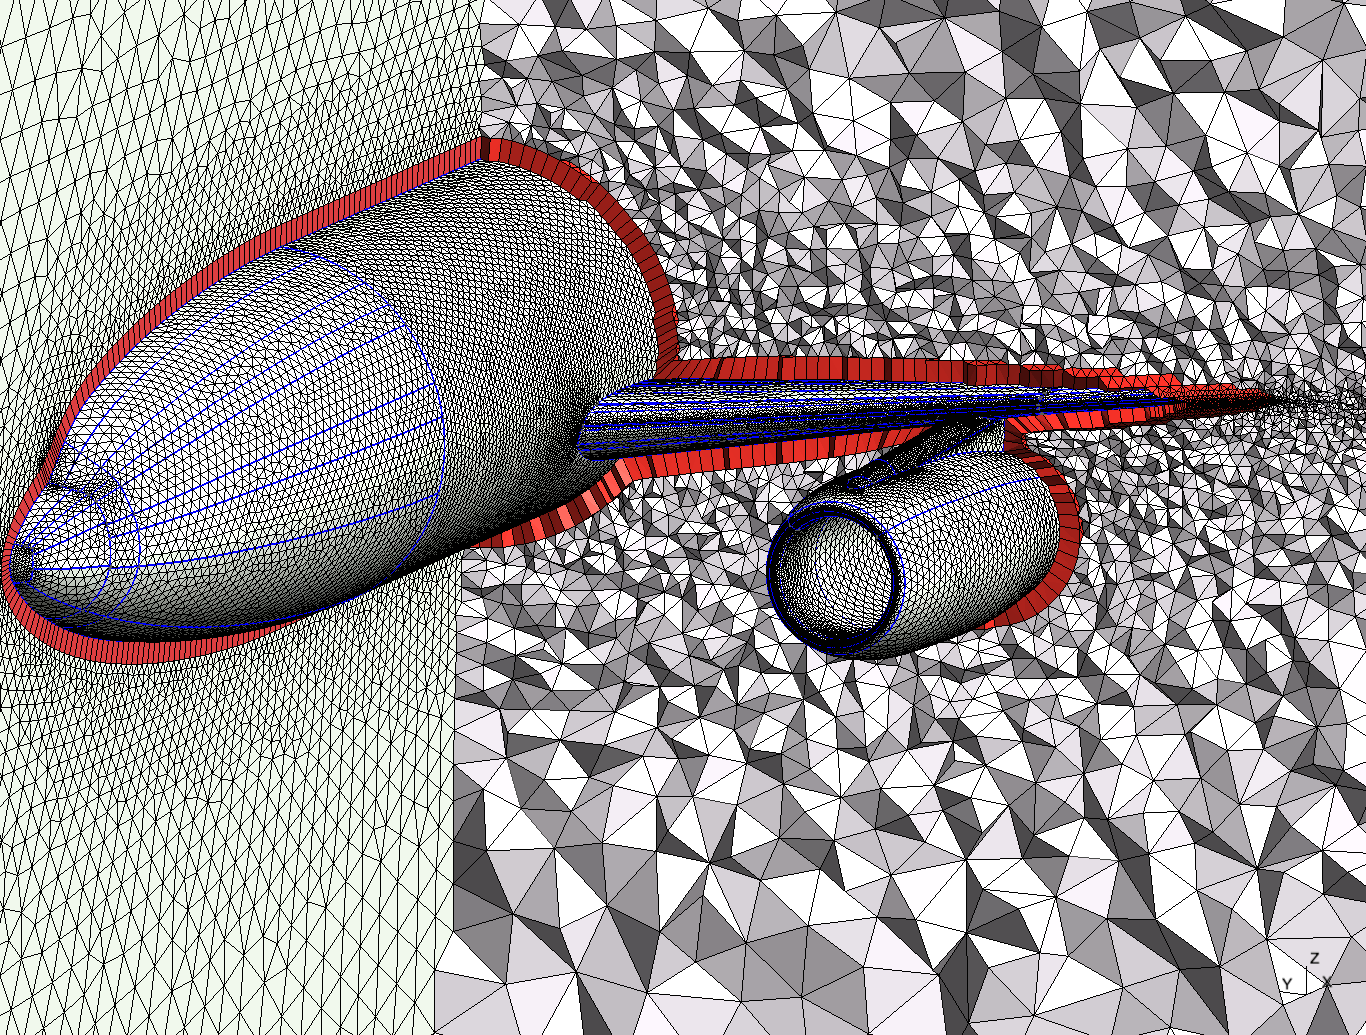
\includegraphics[width=\linewidth]{dlr_f6_1.png}
    \end{column}
    \begin{column}{0.49\textwidth}
      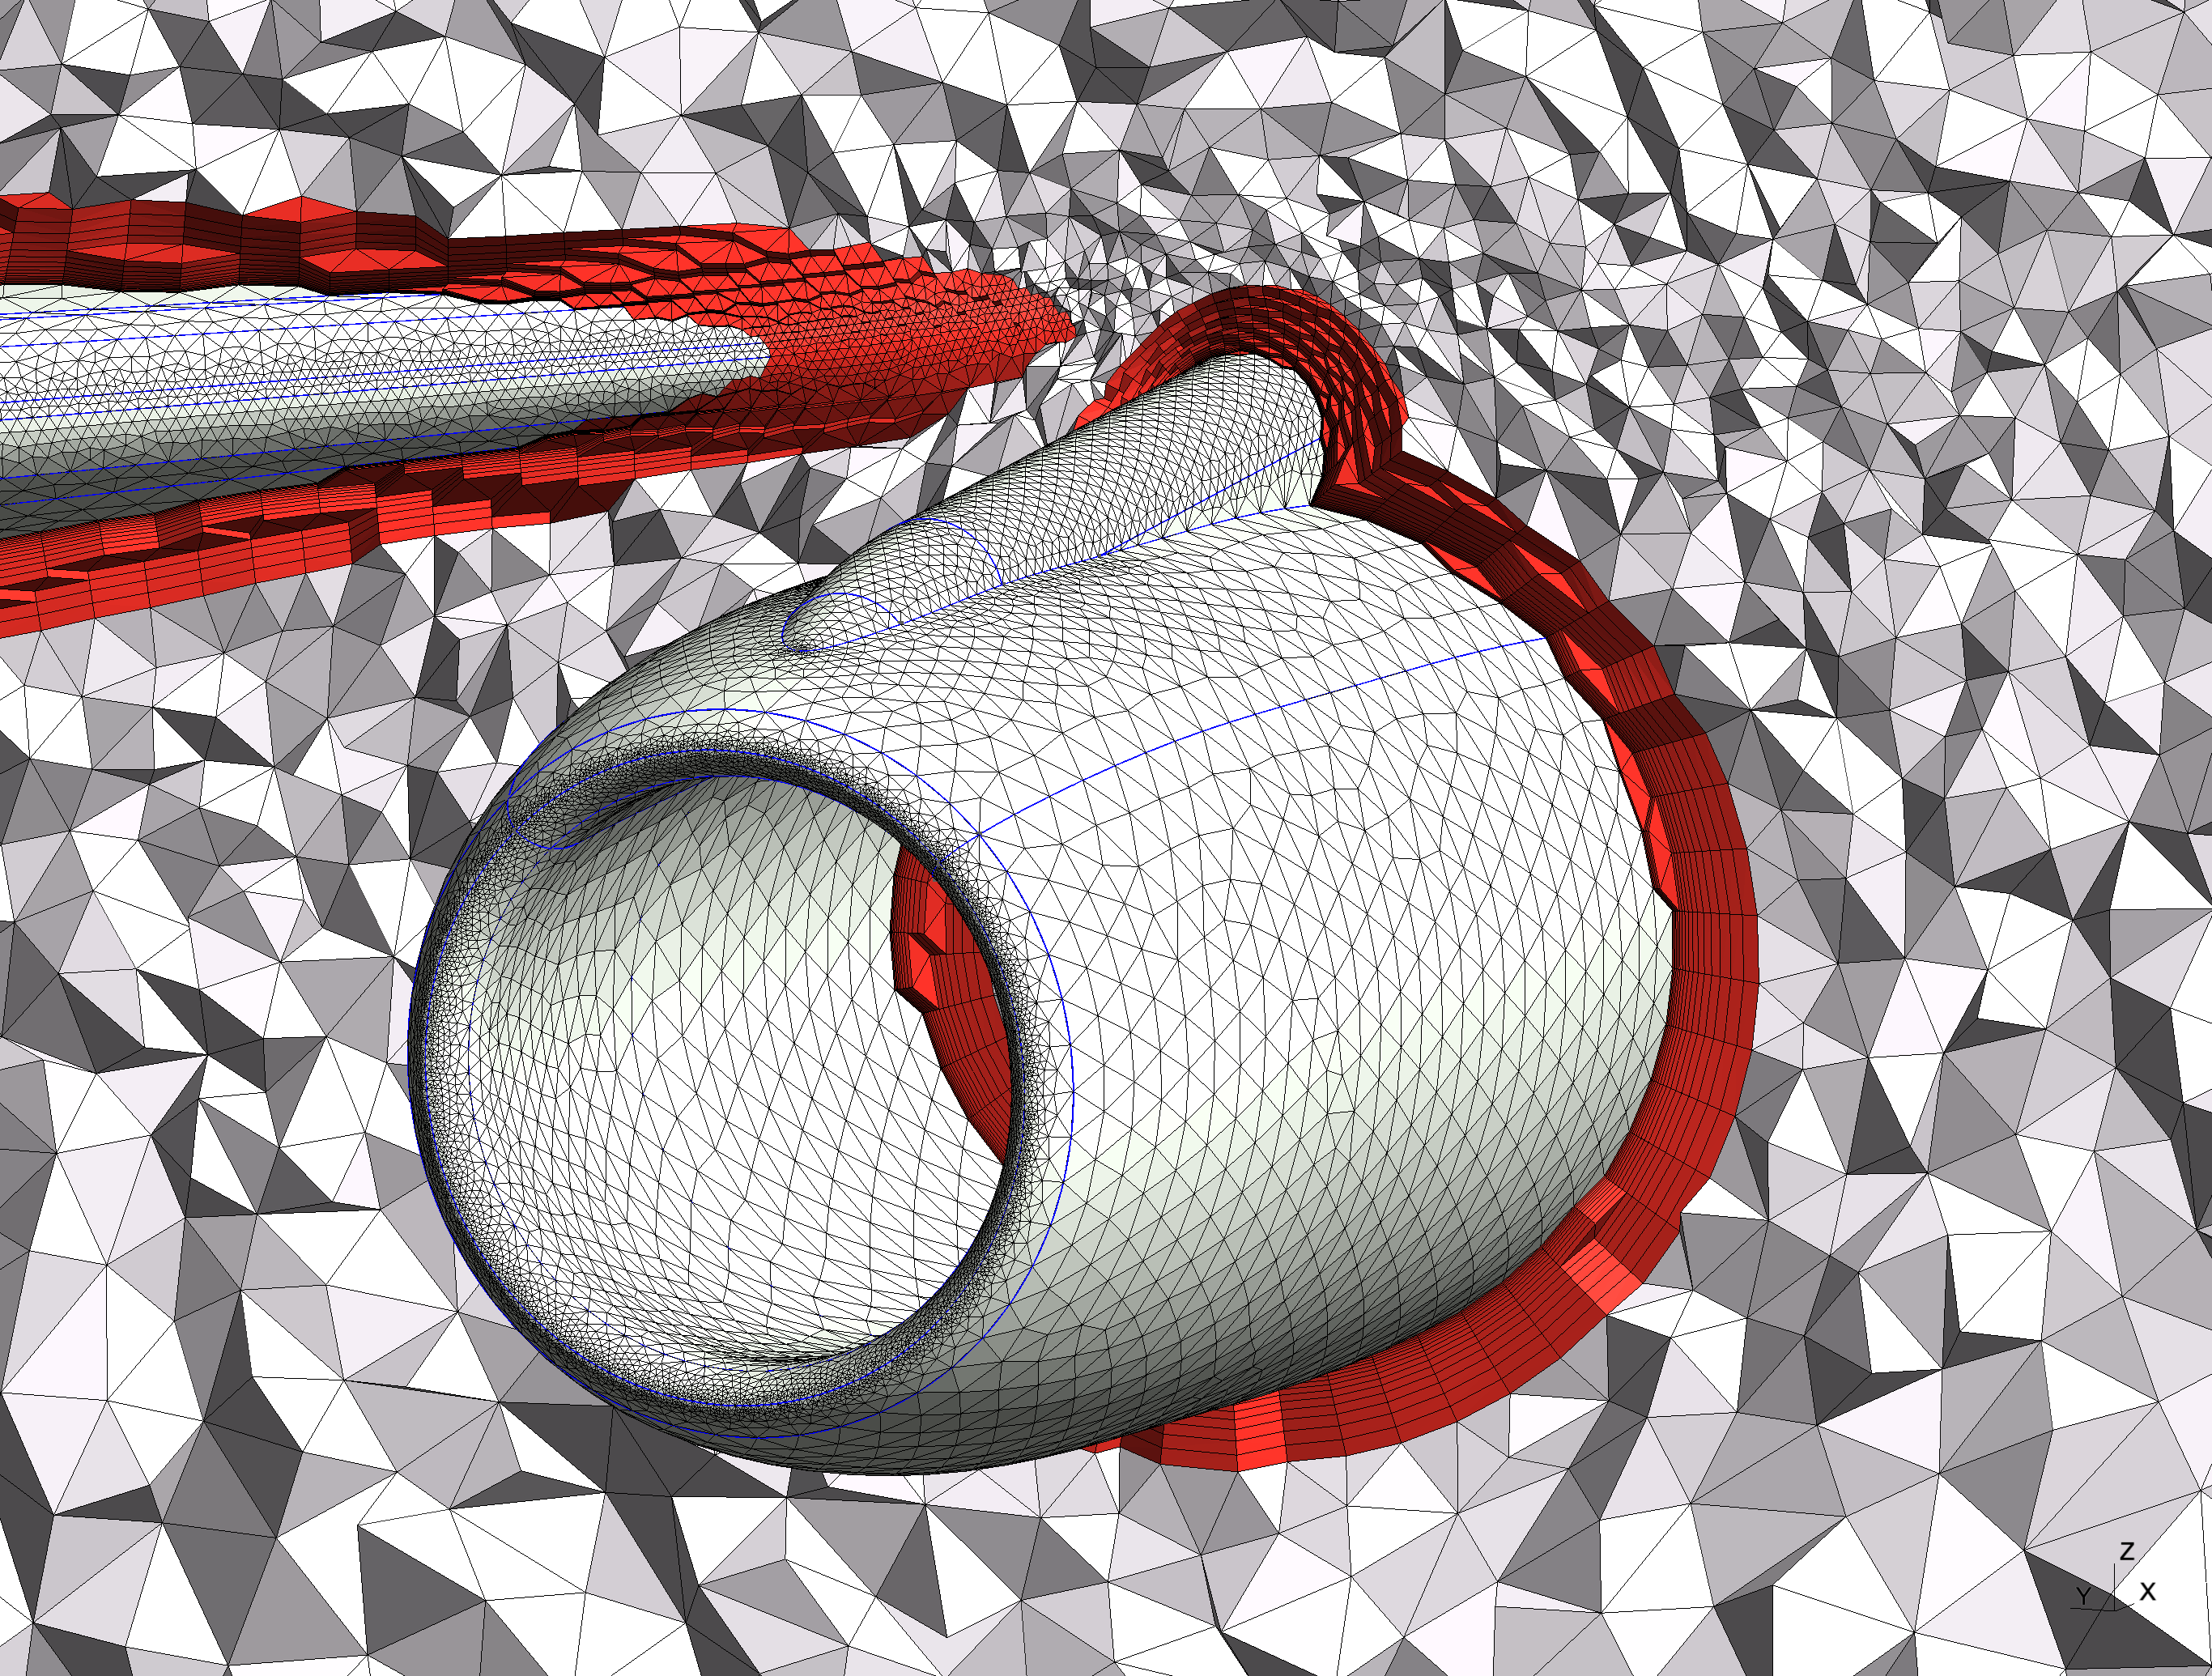
\includegraphics[width=\linewidth]{dlr_f6_2.png}
    \end{column}
  \end{columns}
  \vspace{0.25cm}
  \begin{itemize}
    \item The same plugin flow applies in 3D: selected surfaces support the layer, selected volumes receive it.
    \item The layer can be split into prisms or hexes depending on the topology.
    \item The Winslow push works inside the existing watertight volume mesh.
    \item This makes full-aircraft boundary-layer insertion possible without replacing the Gmsh meshing pipeline.
  \end{itemize}
\end{frame}

\end{document}
